\section{Introduction}

The purpose of this thesis was to design, develop and deploy Smart Travel, a fullstack, cloud-native web platform that empowers travel agencies to compose and sell custom travel packages, while allowing customers to easily search for flights, accommodations, and activities. The primary objective was to solve the main challenges of distributed computing --- namely data consistency across microservices, secure inter-service communication, network latency and deployment automation. The solution implements state-of-the-art industry patterns such as the \textit{Backend-For-Frontend (BFF)}, the \textit{Transactional Outbox} pattern, \textit{Change Data Capture (CDC)}, and \textit{Continuous Integration/Continuous Delivery (CI/CD)} pipelines via Kubernetes-based orchestration.

\section{System Architecture Overview}

To achieve strict separation of concerns and high concurrency, the platform was decomposed into distinct microservices built upon a fully reactive, non-blocking execution model:

\begin{itemize}
    \item \textbf{Travel Catalog API:} Developed with Quarkus to manage travel packages, flights, accommodations, and activities.
    \item \textbf{User API:} Developed with Spring Boot to handle customer profiles and authentication data.
    \item \textbf{Orders API:} Developed with Spring Boot to manage the orders checkout and financial payment workflows.
    \item \textbf{Notification API:} Developed with Quarkus to asynchronously process and dispatch email alerts.
    \item \textbf{API Gateway (BFF):} Developed with Spring Boot to aggregate downstream data from microservices and to secure the API endpoints. It exposes a unified GraphQL interface, abstracting away the underlying RESTful microservice topology and preventing tight coupling between the client and backend services.
\end{itemize}

Beyond the core backend services, the architecture integrates:

\begin{itemize}
    \item \textbf{Database:} To guarantee decoupled persistence, each microservice operates with its own isolated MongoDB database. 
    \item \textbf{Messaging Layer:} For asynchronous, event-driven communication, the system utilizes RabbitMQ as the central message broker, working in conjunction with a Debezium service for Change Data Capture (CDC).
    \item \textbf{Frontend Application:} The client-facing interface is a Single Page Application built with Angular and PrimeNG. It communicates exclusively with the BFF via GraphQL.
\end{itemize}

\begin{figure}[H]
    \centering
    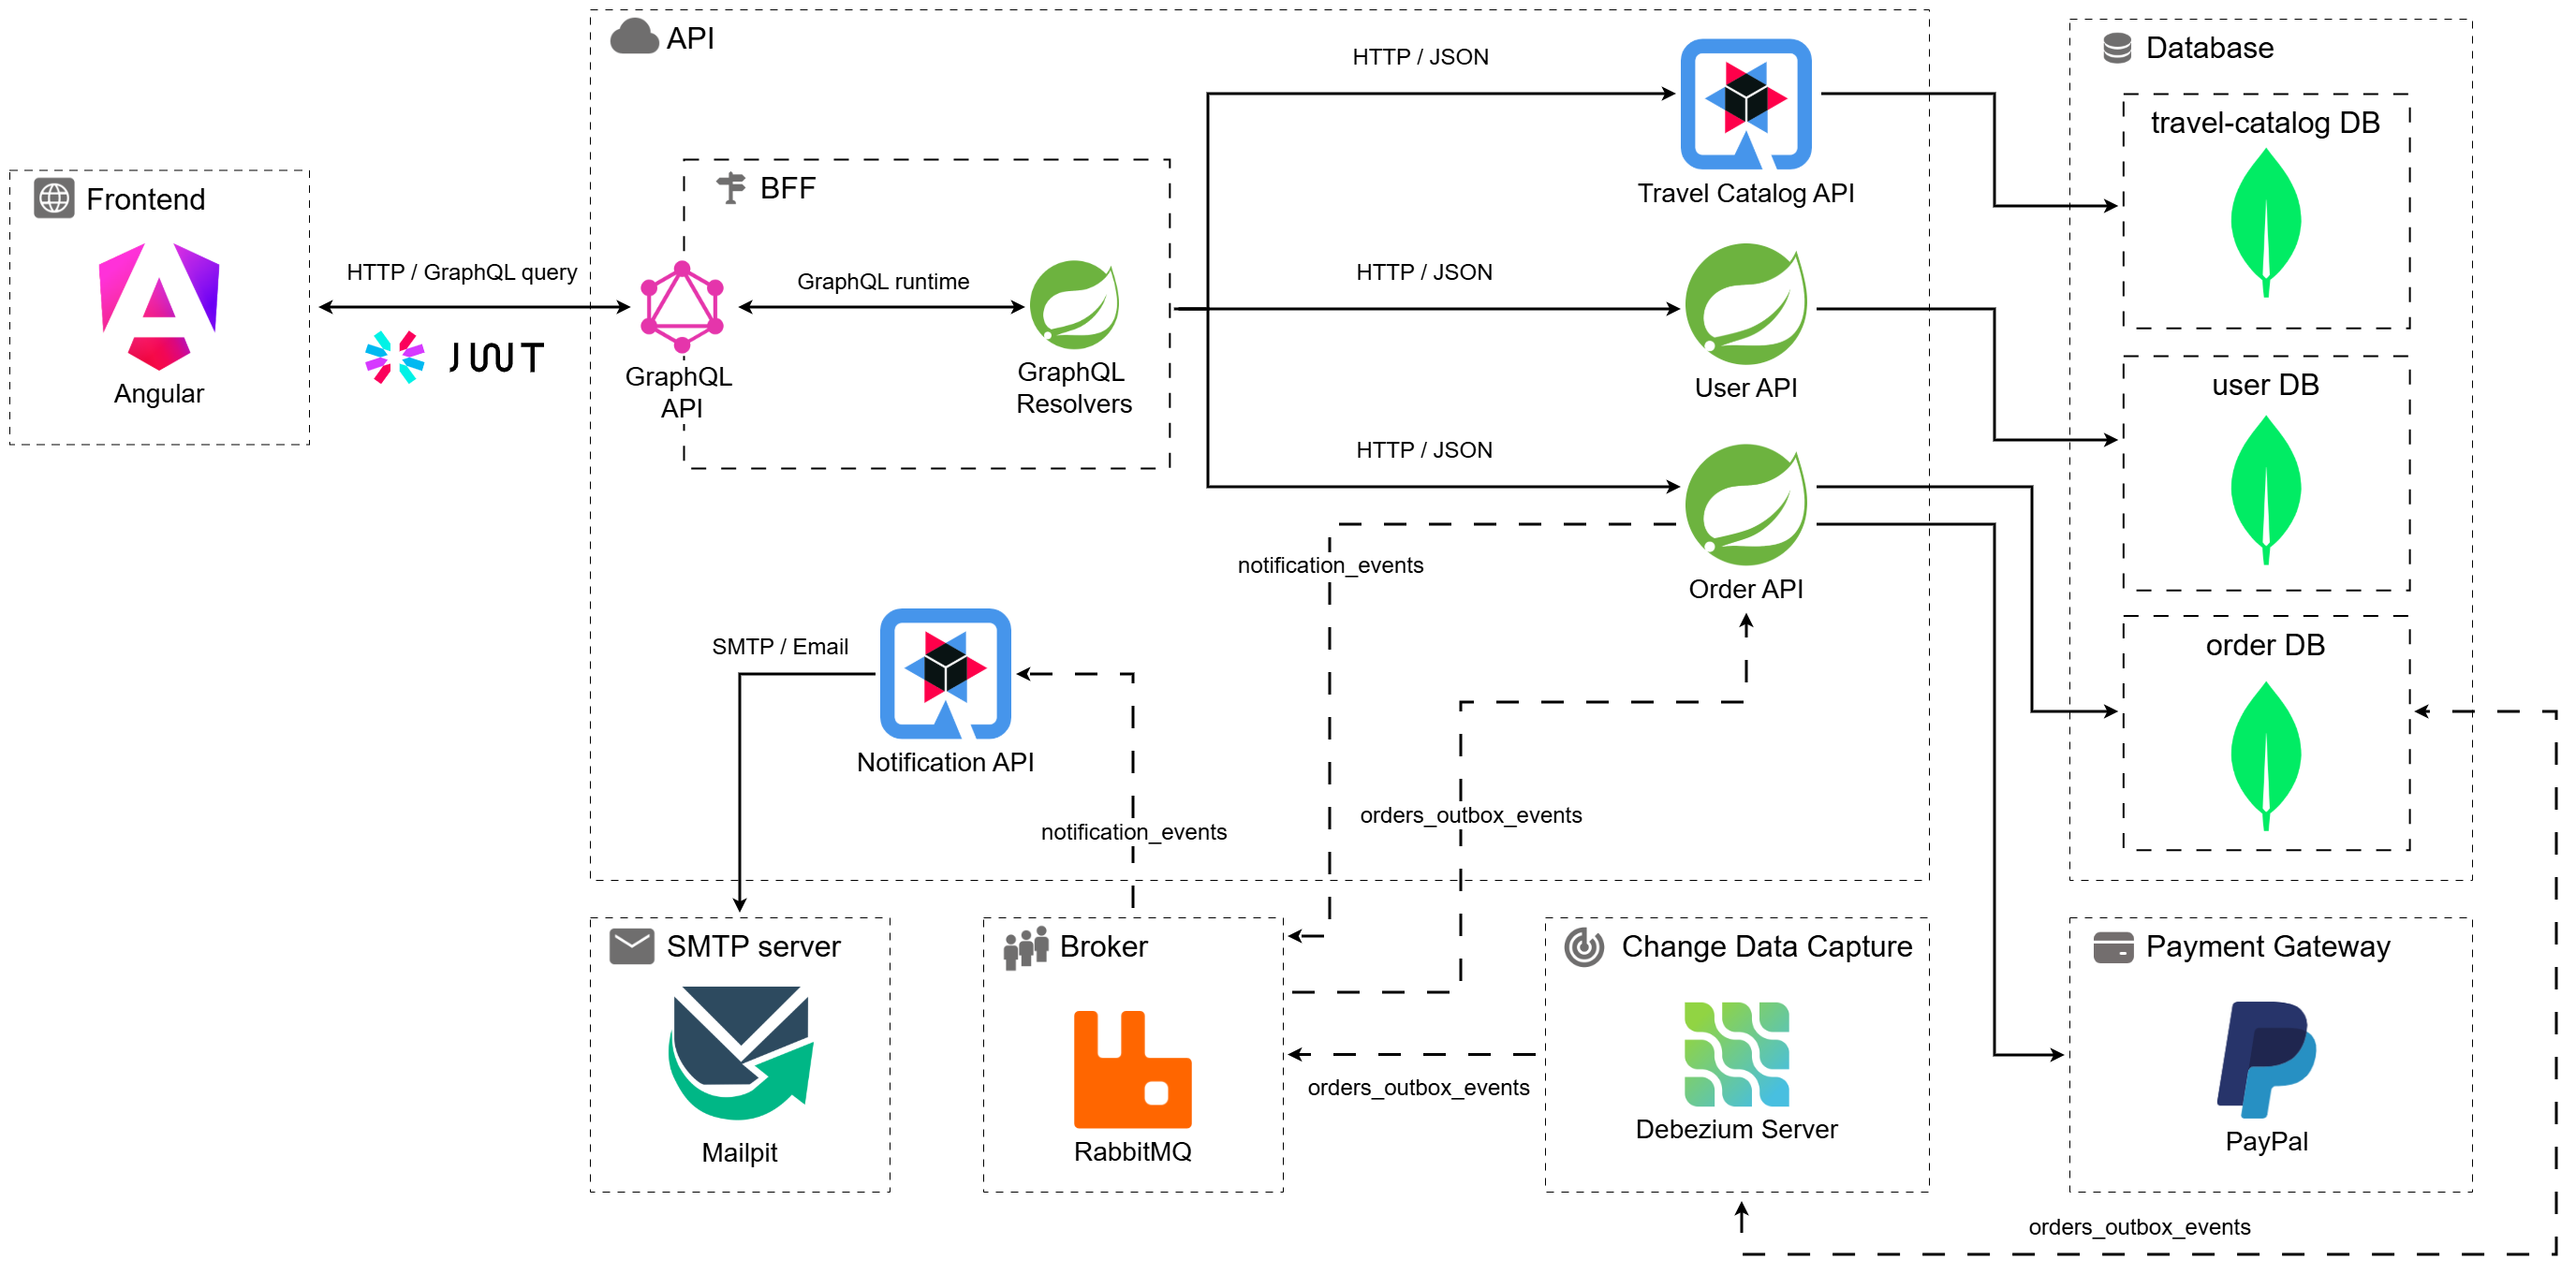
\includegraphics[width=\textwidth]{images/ch3/3_1_architecture-diagram.png}
    \caption[System Architecture]{High-level system architecture of the Smart Travel platform, detailing the microservices topology, the API Gateway and the event-driven messaging layer.}
    \label{fig:system_architecture}
\end{figure}

\section{BFF and Distributed Data Consistency}

To prevent frontend coupling and over-fetching, a BFF was implemented using Spring for GraphQL. It dynamically aggregates downstream data and serves as the primary security perimeter of the application, enforcing Role-Based Access Control (RBAC) using JSON Web Tokens (JWT).

The most complex challenge was maintaining data consistency during the financial checkout phase. To solve this, the platform implements the Transactional Outbox Pattern combined with Change Data Capture (CDC). When a user completes a payment, the event is saved atomically into MongoDB. A standalone Debezium service scans the database operations log (\textit{oplog}) and publishes the event to RabbitMQ. Finally, the Notification API asynchronously consumes the event, guaranteeing at-least-once message delivery.

\section{Infrastructure Automation and Cloud Deployment}

Platform deployment was fully automated via Jenkins declarative pipelines. 

Ephemeral Docker build agents dynamically compile, containerize and securely push container images to an internal OKD (OpenShift) ImageStream registry. The workloads are orchestrated via Kubernetes manifests (\texttt{Deployments}, \texttt{ConfigMaps}, \texttt{Secrets}). For security, the internal microservices are hidden from the public internet; instead, the Nginx frontend container acts as a secure reverse proxy routing traffic to the internal cluster network.

\section{Personal Contribution and Results Obtained}

The architectural design, software engineering, and pipeline automation of the Smart Travel platform were exclusively my personal contributions. Specifically:

\begin{itemize}
    \item \textbf{System Engineering:} Designing the Spring and Quarkus microservices --- including the GraphQL BFF and JWT security layer --- and the frontend Angular SPA.
    \item \textbf{Distributed Systems Integration:} Implementing the Transactional Outbox Pattern, configuring Debezium and establishing the RabbitMQ event-driven architecture.
    \item \textbf{Frontend \& DevOps:} Engineering all the Jenkins CI/CD pipelines and Kubernetes/OKD deployment files.
\end{itemize}

The project resulted in the successful deployment of a highly scalable, fault-tolerant cloud-native platform. The transition to a reactive architecture solved traditional blocking I/O limitations. The BFF eliminated frontend network inefficiencies, while the Debezium/RabbitMQ pipeline guaranteed full data consistency across distributed transactions. Ultimately, the thesis demonstrates that combining modern Java frameworks, reactive programming and DevOps automation successfully produces resilient software capable of meeting dynamic enterprise demands.